\section{Experiments}
In this section, we provide an experimental analysis of the proposed approach to show that layerwise adversarial training improves the performance of the model on the original test data and increases robustness to adversarial inputs. To demonstrate the generality of our training procedure, we present results on CIFAR-10 and CIFAR-100 \cite{krizhevsky2009learning} using VGG, ResNet-20 and ResNet-56 networks. For the ResNet networks, we use the publicly available torch implementation \cite{ResNetTorch}. For the VGG architecture, we use a publicly available implementation which consists of Batch Normalization \cite{VGGTorch}. For all the experiments, we use the SGD solver with Nesterov momentum of 0.9. The base learning rate is 0.1 and it is dropped by 5 every 60 epochs in case of CIFAR-100 and every 50 epochs in case of CIFAR-10. The total training duration is 300 epochs. We employ random flipping as a data augmentation procedure and standard mean/std preprocessing was applied conforming to the original implementations. For the ResNet baseline models, without regularization, we find that they start overfitting if trained longer and hence we perform early stopping and report their best results. For the perturbed models, we find that no early stopping is necessary; the learning continues for a longer duration and shows good convergence behavior.  We refer to the model trained using the proposed approach described in Algorithm \ref{tab:algo} as $Perturbed$ throughout this section. Dropout was not used in any of the training procedure in this experiment. We explicitly compare our approach against dropout in the ablative experiments. Figure \ref{fig:train_example} plots the training and test error rates for the baseline model and the proposed approach. It can be observed that our method converges faster and achieves better generalization error. Note that, we used  only random shuffling in all our experiments since we found that performing a controlled shuffling to improve mini-batch overlap across i. and hence we use


\begin{table}[!h]
\caption{Classification accuracy (\%) on CIFAR-10 and CIFAR-100 for VGG and Resnet architectures. Results reported are average of 5 runs.}
\label{tab:cifar-results}
 \begin{tabular}{||c | c | c ||} 
 \hline
 Type (CIFAR-10) & Baseline & Perturbed \\ [0.5ex] 
 \hline
 VGG  & 92.1 $\pm$ 0.3 & 92.65 $\pm$ 0.2 \\ 
 \hline
 Resnet-20 & 90.27 $\pm$ 0.4 & 91.1 $\pm$ 0.3 \\
 \hline  
 Resnet-56 & 91.53	$\pm$ 0.3 & 94.1 $\pm$ 0.2 \\
 \hline 
\end{tabular}
\quad 
\begin{tabular}{||c | c | c ||} 
 \hline
 Type (CIFAR-100) & Baseline & Perturbed \\ [0.5ex] 
 \hline
 VGG  & 69.8 $\pm$ 0.5 & 72.3 $\pm$ 0.3  \\ 
 \hline
 Resnet-20 & 64.0 $\pm$ 0.2 & 66.9 $\pm$ 0.3 \\
 \hline
 Resnet-56 & 68.2 $\pm$ 0.4 & 71.4 $\pm$ 0.5 \\
 \hline
\end{tabular}
\end{table}

\begin{figure*}[!h]
  \centering
  \subfloat[CIFAR-10]{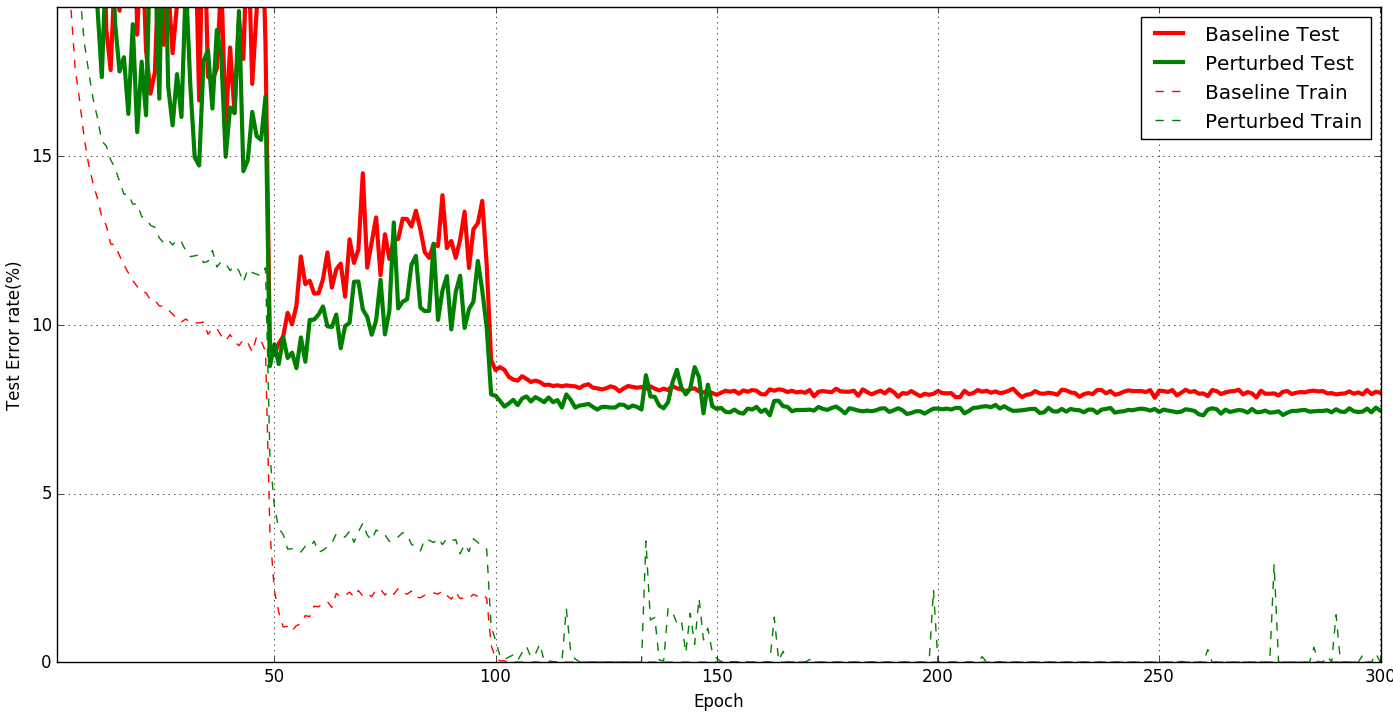
\includegraphics[width=0.4\textwidth,height=0.2\linewidth]{cifar10-vgg-nodrop-flip.png}}   
   \subfloat[CIFAR-100]{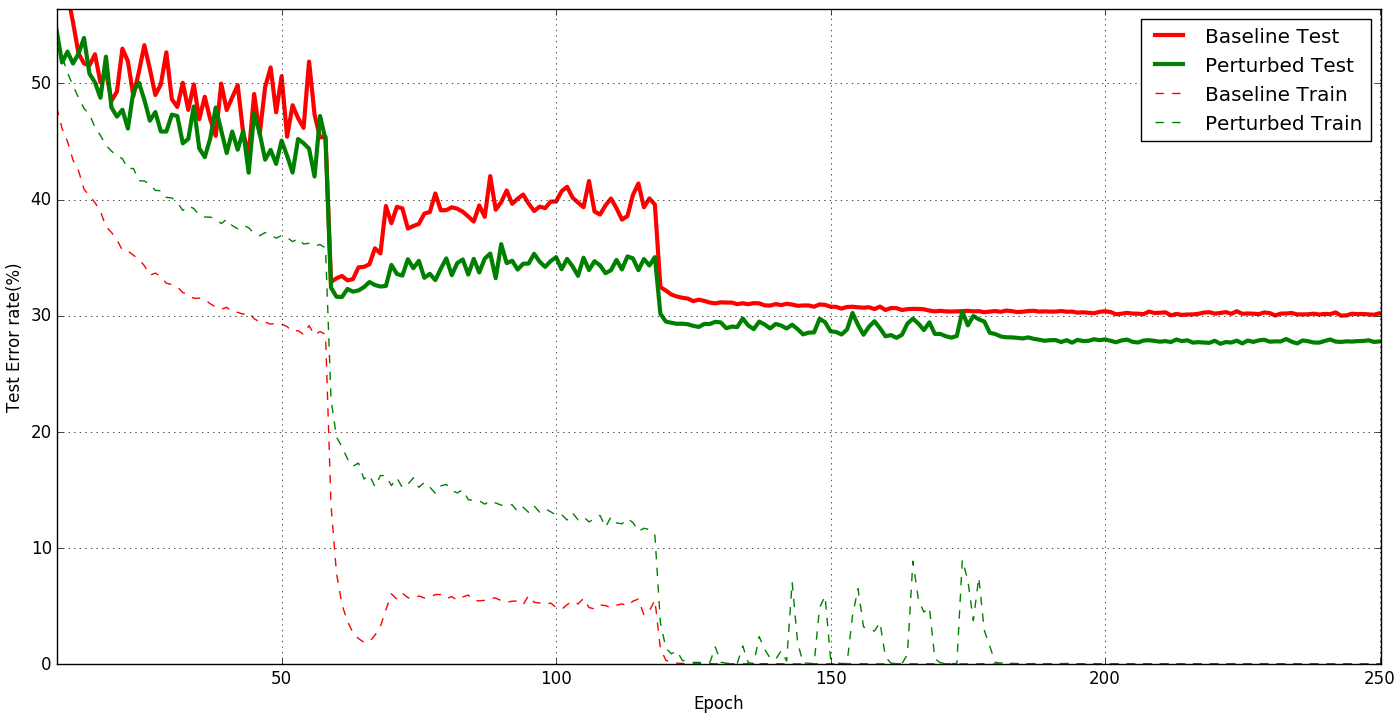
\includegraphics[width=0.4\textwidth,height=0.2\linewidth]{cifar100-vgg-nodrop-flip.png}}  
  \caption{Training and test error rates for VGG network trained on CIFAR-10 and CIFAR-100 datasets. The training errors are computed using  perturbed activations in each epoch. The red color indicates the baseline model and green indicates the model regularized with the proposed approach, referred as \textit{Perturbed} in the text. Best viewed in color. Please zoom in for clarity.}
  \label{fig:train_example}
\end{figure*}

\textbf{Imagenet Experiment:} To test the applicability of our regularization approach over a large scale dataset, we conducted an experiment using the ImageNet dataset (train: 1.2M images, val: 50K images). We used AlexNet as the base architecture. We used the publicly available implementation from the torch platform \cite{AlexnetTorch} and both the baseline and the regularized models were trained from scratch to 60 epochs. The classification accuracies obtained were: Baseline - 56.1\%, Proposed - 59.2\%, an increase of 3.1\%. This shows that our approach can significantly improve the performance of deep neural networks even on a large and diverse corpus like Imagenet.

% \textbf{Note on data shuffling:} As mentioned in our formulation, we employ random shuffling when training our models. However, one can argue that the performance of the proposed approach can be improved by performing a controlled data shuffling at each iteration such that there is no class label overlap between successive mini-batches. We found that this did not yield statistically significant improvement in performance and hence we use only random shuffling in all our experiments. This can be explained by our observation that even with random shuffling the overlap between successive batches was $\sim$3\% for CIFAR-10 dataset and it was even lesser for the CIFAR-100 and ImageNet datasets. We would like to note here that in a setting where the training dataset has a severely unbalanced distribution, an inexpensive data shuffling strategy can be employed once before training begins or at the beginning of each epoch to ensure no overlap. 

% In our approach, since we rely on gradients from the previous batch of inputs, there could be a class label overlap between the current batch and the previous batch. To measure the amount of overlap, we performed several monte carlo simulations where we randomly shuffle the training data and measure class overlap across successive batches.  We observed that the probability of such overlap on the datasets used in our experiments was negligible and hence, did not have any impact on our performance. If a different dataset has a severely unbalanced distributions, an inexpensive data shuffling strategy can be employed once before training begins or at the beginning of each epoch to ensure no overlap. In our experiments, we observed that randomly shuffling the data yielded the same performance as using controlled shuffling to ensure no overlap.

% To test whether such overlap has any effect on our performance, we did try explicit reshuffling ensuring no overlap between successive mini-batches before each epoch. However, we did not observe any improvement in performance compared to performing only random shuffling. For severely unbalanced distributions, an inexpensive data shuffling strategy can be employed once before training begins or at the beginning of each epoch.

\section{Ablative Experiments and Discussion}

\textbf{Comparison with Dropout:} We perform an experiment where we compare the regularization performance of the proposed adversarial training approach to Dropout. We use the VGG architecture used in the previous sections and perform experiments with and without dropout on CIFAR-10 and CIFAR-100 datasets. 
%To understand the full extent of the regularization performance, we did not perform any data augmentation for this experiment. 

\begin{center}
\captionof{table}{Comparison of classification accuracy (\%) with/without dropout on CIFAR-10 and CIFAR-100 for the VGG model}
\label{tab:dropout-results}
 \begin{tabular}{||c | c | c ||} 
 \hline
 Type (CIFAR-10) & Baseline & Perturbed \\ [0.5ex] 
 \hline
 w/o Dropout & 92.1 & 92.7  \\ 
 \hline
 with Dropout & 92.5 & 93.2 \\
 \hline  
\end{tabular}
\quad 
\begin{tabular}{||c | c | c ||} 
 \hline
 Type (CIFAR-100) & Baseline & Perturbed \\ [0.5ex] 
 \hline
 w/o Dropout & 69.8 & 72.3  \\ 
 \hline
 with Dropout & 70.5 & 73.1 \\
 \hline  
\end{tabular}
\end{center}

The following observations could be made from Table \ref{tab:dropout-results}: (1) The perturbed model performs better than the baseline model with or without dropout. Thus, the proposed training improves the performance of even dropout based networks. (2) On a complex task like CIFAR-100, the proposed adversarial training based regularization gives better performance compared to that provided by dropout (70.5\% (vs) 73.1\%). Since the proposed adversarial perturbations are intended to move the inputs towards directions that strongly resist correct classification, they are able to create a more discriminative representation for tasks with a larger number of classes. 

\begin{center}
\captionof{table}{Effect of adding gradient accumulation layers incrementally (from shallow to deeper layers) throughout the deep network. The numbers reported are the classification accuracy using the VGG network on the CIFAR-10 dataset. Baseline performance is 89.4\%. \textit{conv1 to} indicates we start adding the gradient accumulation layers from \textit{conv1} upto the mentioned layers such as \textit{pool1}, \textit{pool2} etc.}
\label{tab:layerwise}
\resizebox{.45\textwidth}{!}{%
 \begin{tabular}{||c | c | c | c | c | c ||} 
 \hline
 Layer (conv1 to) & pool1 & pool2 & pool3 & pool4 & pool5\\ [0.5ex] 
 \hline
 Accuracy & 89.5 & 89.62 & 90.24 & 91.1  & 91.3  \\
 \hline  
\end{tabular}
}
\end{center}

\textbf{Perturbing deeper layers:} In this section, we analyze the effect of adversarial perturbations starting from the lowest convolutional layers which model edges/shape information to the more deeper layers which model abstract concepts. For this experiment, we use the VGG network with batch normalization that was used in the previous section. The experiments were performed on the CIFAR-10 dataset. No data augmentation or dropout is applied. It is clear from the results in Table \ref{tab:layerwise} that the improvement in performance due to the proposed layerwise perturbations become significant when applied to the deeper layers of the network, which is in line with the observation made by \cite{szegedy2013intriguing}. While performing layerwise alternate training as proposed by\cite{szegedy2013intriguing}  becomes infeasible for even moderately deep architectures, our training scheme provides an efficient framework to infuse adversarial perturbations throughout the structure of very deep models. 


\begin{table}
\centering
\captionof{table}{Comparison of the strength of adversarial examples between the FGS approach applied at the input and using the proposed layerwise perturbations. Reported numbers are classification accuracies for different values of $\epsilon$.}
\label{tab:compare_adv}
\resizebox{0.45\textwidth}{!}{%
 \begin{tabular}{||c | c | c | c | c | c ||} 
 \hline
 Type & $\epsilon=0$ & $\epsilon=0.05$ & $\epsilon=0.1$ & $\epsilon=0.15$ & $\epsilon=0.2$ \\ [0.5ex] 
 \hline\hline
 FGS \shortcite{goodfellow2014explaining}  & 92.4 & 53.28 & 41.58 & 36.44 & 33.85  \\ 
 \hline
%  Ours - only input & 92.4 & 92.35 & 92.29 & 92.04 & 90.91 \\
%  \hline 
 Ours - all layers & 92.4 & 48.56 & 21.72 & 14.76 & 14.19 \\
 \hline
\end{tabular}
}
\vspace{-2mm}
\end{table}
\textbf{Adversarial strength of the proposed perturbations:} Traditional adversarial training techniques improve the performance on adversarial examples by explicitly making the network robust to adversarial gradient directions. Thus, an important question that needs to be addressed in light of the proposed optimization strategy is: Are the gradient directions generated from the previous samples(as described in Algorithm 1) adversarial ? To answer this question, we perform an empirical experiment to measure the performance of a deep model (3 convolutional layers + 1 fc-layer) trained using CIFAR-10 training data, on the CIFAR-10 test data. No adversarial training was used to train this model. As described earlier, for each test sample, the intermediate layer activations are perturbed using gradients accumulated from the previous sample. For comparison, we also show the performance of the same model on the adversarial data generated using the FGS method. From the metrics in Table \ref{tab:compare_adv}, it can be observed that using accumulated gradients from the previous batch as adversarial perturbations results in a bigger drop in performance. This signifies that the aggregated effect of layerwise perturbations is more adversarial compared to perturbing only the input layer as done in the FGS approach. We performed an additional experiment where only the input layer was perturbed using the gradients of the previous sample instead of perturbing all the intermediate layers. We found that this resulted in negligible drop in the baseline performance, indicating that these gradients are not adversarial enough when used to perturb only the input. 

\begin{table}[b!]
\begin{center}
\captionof{table}{Comparison of classification accuracy (\%) between the different variants of the proposed approach and FGS method (FGS-orig) for different values of $\epsilon$}
\label{tab:variants}
\resizebox{.45\textwidth}{!}{%
 \begin{tabular}{||c | c | c | c | c | c | c ||} 
 \hline
 Type & $0$ & $0.02$ & $0.04$ & $0.06$ & $0.08$ & $0.1$ \\
 \hline
 Baseline & 89.4 & 67.5 & 49.6 & 41.2 & 37.3 & 34.7   \\
 \hline  
 FGS-orig \shortcite{goodfellow2014explaining} & 88.7 & 86.4 & 84.1 & 81.4 & 80.5 & 77.1  \\
 \hline  
 FGS-inter & 90.9 & 87.79 & 83.85 & 79.65 & 74.69 & 69.92 \\
 \hline  
 Ours-orig & 91.2 & 87.95 & 83.84 & 79.11  & 73.66 & 68.37  \\
 \hline  
 Ours-joint & 91.5 & 86.07 & 81.38 & 75.72 & 70.25 & 64.76  \\
 \hline  
\end{tabular}%
}
\end{center}
\end{table}

% \begin{table*}
% \begin{center}
% \captionof{table}{Comparison of classification accuracy (\%) between various training approaches described in Section \ref{subsec:variants}}
% \label{tab:variants}
%  \begin{tabular}{||c | c | c | c | c | c | c | c ||} 
%  \hline
%  Type & $\epsilon=0$ & $\epsilon=0.02$ & $\epsilon=0.04$ & $\epsilon=0.06$ & $\epsilon=0.08$ & $\epsilon=0.1$ & Training time \\ [0.5ex] 
%  \hline
%  Baseline & 89.4 & 67.5 & 49.6 & 41.2 & 37.3 & 34.7  & x \\
%  \hline  
%  FGS-orig & 88.7 & 86.4 & 84.1 & 81.4 & 80.5 & 77.1  & 2x \\
%  \hline  
%  FGS-inter & 90.9 & 87.79 & 83.85 & 79.65 & 74.69 & 69.92  & 2x \\
%  \hline  
%  Ours-orig & 91.2 & 87.95 & 83.84 & 79.11  & 73.66 & 68.37  & x \\
%  \hline  
%  Ours-joint & 91.5 & 86.07 & 81.38 & 75.72 & 70.25 & 64.76  & 2x \\
%  \hline  
% \end{tabular}
% \end{center}
% \end{table*}

\textbf{Variants of the proposed approach:}\label{subsec:variants} In the proposed training method summarized in Algorithm \ref{tab:algo} (referred as Ours-orig), each batch of inputs is perturbed at intermediate layers by the gradients accumulated from the previous batch. In this section, we present an empirical comparison between the following variants:
\begin{itemize}
\item FGS-orig: The original FGS joint loss based adversarial training as proposed by \cite{goodfellow2014explaining} and shown in Eq. (\ref{eq:fgs_train}). We used a value of $\alpha=0.5$; we did not find other values yield any significant improvements. %Following the original approach, the FGS perturbations are only used at the input.
\item FGS-inter: In this setting, different from \cite{goodfellow2014explaining}, we use the FGS gradients to perturb the intermediate layer activations and use the joint loss with $\alpha=0.5$.
\item Ours-joint: This setting is same as Ours-orig with the exception that we use the joint loss formulation with $\alpha=0.5$. Note that, Ours-orig corresponds to setting where $\alpha=0$
%critical difference being that the adversarial perturbations are gradients from the previous batch, similar to Ours-orig.
\end{itemize}
All the models are trained on the CIFAR-10 dataset. No data augmentation or dropout regularization is applied. The training parameters are similar to the ones used in the previous section. We generate adversarial test data for the CIFAR-10 test dataset using the FGS method, since it has been shown to generate adversarial examples reliably. We then test the models on the original and adversarial test data for different values of the adversarial strength $\epsilon$. Table \ref{tab:variants} shows the results of the different training strategies. $\epsilon=0$ corresponds to the original test data and other values of $\epsilon$ indicate the strength of adversarial FGS perturbation added to the input image. From these results, we make the following observations: (1)  Approaches based on perturbing intermediate layers (FGS-inter,Ours-orig,Ours-joint) improve the performance on the original data significantly as compared to perturbing only the input but they marginally decrease the adversarial test performance. (2) On the other hand, perturbing only the input layer (FGS-orig) yields the best adversarial test performance among the compared approaches while performing marginally worse than the baseline on the original test data. These observations indicate the possibility of a trade-off that exists between adversarial robustness and regularization effect over clean data. Referring to the toy example described earlier, the singular value analysis performed there also supports our claim that methods which impart adversarial robustness tend to suppress sensitivity of the model in all the dominant directions; while the proposed approach provides a nice trade-off by retaining those directions which are essential for modeling the variations in the training data. This ensures that our approach results in better regularization performance on clean data while providing comparable robustness on adversarial data.

\textbf{Results on WideResNet models:} Wide Residual Networks are recently proposed deep architectures that generated state of the art results on CIFAR-10 and CIFAR-100 datasets. In this experiment, we use their publicly available implementation and train them from randomly initialized weights using the proposed approach using the parameter settings described in the experiments section. Specifically, the Ours-joint approach described in the previous section is used for training. As data augmentation, we applied flipping and random cropping as done in their native implementation. The results are shown in Table \ref{tab:cifar-results}. For the compared methods, we quote their published accuracy values. It can be observed that the proposed approach results in improved performance compared to both the baseline model and the model regularized with dropout. This demonstrates the generalization ability of our approach to state of art deep models. 
\begin{center}
\captionof{table}{Classification error rates (\%) on CIFAR-10 and CIFAR-100 for WideResNet (WRN) architectures. Our results are reported as average of 5 runs. For comparison we provide the published WRN baseline results. $^{(*)}$ denotes the results obtained by a single run.}
\label{tab:cifar-results}
\resizebox{.45\textwidth}{!}{%
 \begin{tabular}{| c | c | c | c |} 
 \hline
 Model & \#params & CIFAR-10 & CIFAR-100 \\ [0.5ex] 
 \hline
 WRN-28-10 \shortcite{wideresnet} & 36.5M &  4.00 & 19.25\\ 
 \hline
 WRN-28-10 with dropout \shortcite{wideresnet}  & 36.5M &  3.89 & 18.85\\ 
 \hline
 WRN-40-10 with dropout$^{*}$ \shortcite{wideresnet}  & 51.0M &  3.8 & 18.3\\ 
 \hline
 WRN-28-10 - \textbf{Ours} & 36.5M & \textbf{3.62} $\pm$ 0.05 & \textbf{17.1} $\pm$ 0.1 \\
 \hline  
\end{tabular}
}
\end{center}

\textbf{Generalization to non-image signals:}
In this work, we have considered adversarial perturbations in the space of natural images. The existence of adversarial perturbations has been shown to exist in other types of signals that occur in speech recognition (\cite{serdyuk2016invariant}, \cite{carlini_speech}) and language processing tasks \cite{miyato_NLP}. While the focus of the this paper has been image signals, there exists a natural extension of our framework to the above modalities. Such an extension is trivially possible since end-to-end learning systems such as deep networks are used in speech and language tasks as well. As future work, we propose to extend the current approach to explore robustness aspects of deep networks trained on modalities other than images.

% On the original test data, it can be clearly observed that our approach improves upon both the baseline and FGS-orig. Looking closely into the other columns, we see that FGS-orig provides an improved performance on the adversarial test data. Overall, we can observe that the proposed approach Ours-orig provides significant gain in original performance while providing comparable adversarial robustness. 


% \textbf{This indicates a trade-off that exists between adversarial robustness and classification performance. The objective of contemporary methods for adversarial training is to maintain the original performance while improving adversarial robustness. Our proposed approach . This trade off is more fundamental and explored in recent theoretical works on robustness in a more detailed manner.This tradeoff is again evident when we compare the FGS-orig and FGS-inter approaches.} The adversarial perturbations when added to the intermediate layers offer additional regularization benefit while still providing robustness against adversarial examples. By comparing Ours-orig and FGS-inter, we see that the proposed approach is more efficient and provides the same or better results as the FGS-inter approach. This is more clearly observed by observing the results of the Ours-joint approach which provides the best baseline performance in Table \ref{tab:variants}.

%This empirical observation demonstrates that perturbing inputs or perturbing intermediate layers have opposing implications for the performance of the learning algorithm on original and adversarial test data.



% \begin{figure}[!h]
%   \centering
%   \subfloat[Adversarial performance with dropout]{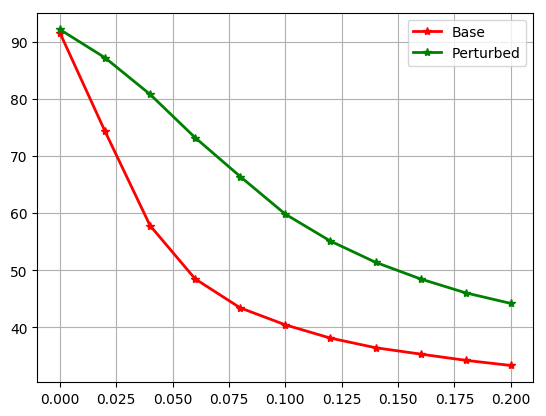
\includegraphics[width=0.4\textwidth]{cifar10_vgg_adv_test_dropout.png}\label{fig:f1}}
%   \hfill
%   \subfloat[Adversarial performance without dropout]{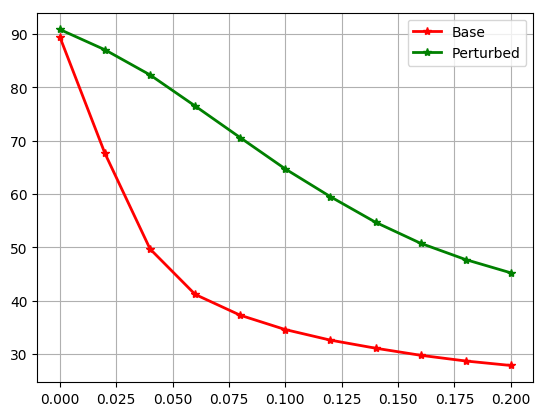
\includegraphics[width=0.4\textwidth]{cifar10_vgg_adv_test_no_dropout.png}\label{fig:f2}}
%   \caption{Performance comparison of the baseline and perturbed networks on the CIFAR-10 test data.}
%   \label{fig:adv_test}
% \end{figure}

% \subsection{Performance on Adversarial test data}
% While the previous results show that ELAT acts as a strong regularizer, in this section we validate our claim that the models trained using ELAT make the network more robust to adversarial examples. We setup a simple experiment to validate this claim by generating adversarial test data for the CIFAR-10 test dataset using the FGS method, since it has been shown to generate adversarial examples reliably. We then test the baseline model and the perturbed model on the adversarial test data. To provide a more thorough comparison, we also vary the value of $\epsilon$ that is used to generate the adversarial examples. 

% Figure \ref{fig:adv_test} shows the results for testing on adversarial examples generated from the test set of 10000 datapoints. It is clear from the plots that the ELAT makes the network more robust to adversaries. It should be noted that the input layer is not perturbed during training rather only the intermediate layers are perturbed. Hence, the space of these adversarial examples have not been explicitly explored by the model during training. 

% \subsection{Wideresnet performance}
% We apply the joint adversarial training approach to the wideresnet architecture which have been shown to produce very high accuracy on the CIFAR-100 dataset. In order to evaluate the practical utility of our approach we apply the same training parameters and data augmentation techniques as the baseline implementation. We train our model for 250 epochs dropping the learning rate every 60 epochs by 5.  
% \subsection{runtime analysis}
% Since we are talking about efficient training, we should discuss runtime analysis.
